% IEEE konferans şablonu (dersin verdiği şablonla değiştirilebilir). Overleaf'te derlenir.
% Sayılar: analysis/summary.md (çekirdek), analysis/summary_evo.md (evrimsel katman).
\documentclass[conference]{IEEEtran}
\usepackage[utf8]{inputenc}
\usepackage[T1]{fontenc}
\usepackage[turkish]{babel}
\usepackage{amsmath,graphicx,booktabs,cite}
\graphicspath{{../analysis/figures/}{../experiments/results/}}

\begin{document}
\title{Yaradan Doğan Çeşitlilik:\\ Genom Koşullu Nöral Hücresel Otomatlarla Planarya Benzeri Bir Ekosistemde Yenilenme ve Evrim}
\author{\IEEEauthorblockN{Arda}}
\maketitle

\begin{abstract}
Tüm hücrelerin paylaştığı tek bir öğrenilmiş yerel kural (NCA) ile kalıtsal bir genomun biçimi belirlediği, planarya benzeri canlılardan oluşan bir ekosistem kuruyoruz. Kesilen canlının yarasında bir potansiyel oluşur ve genom orada mutasyona uğrar; parçalanma üremedir ve canlılar sınırlı kaynak için rekabet eder. Çekirdek katmanda tek hedefli NCA ile büyüme, onarım ve parça boyutu--yenilenme eğrisini ölçüyor, kesme eğitimi olmadan bölünmenin dairesel onarım eğitiminden kendiliğinden çıktığını gösteriyoruz. Evrimsel katmanda ata fiziği, eğitimde görülmemiş genomların \%100'ünde yaşayabilir canlılar üretir (hedefine IoU 0,967); soylar arasında yüksek kalıtsal uygunluk farkı vardır ($H^2 = 0{,}72$) ve popülasyon uygunluğu 30\,000 adımda \%30--40 artar. Yüksek mutasyon hızı ($\mu = 1$) uyumu yaklaşık iki kat hızlandırır; yara mutasyonu kuruculardan uzak, kurucu düzeyinde uygun yeni genomlar üretir, ancak 30\,000 adımda en iyi kurucunun ötesine geçen bir yenilik istatistiksel olarak gösterilemedi ($p \approx 0{,}08$).
\end{abstract}

\section{Giriş}
% Levin'in biyoelektrik desen hafızası, Durant vd.~\cite{durant2017longterm}; Mordvintsev vd.~\cite{mordvintsev2020growing}.
% Soru: hedef görüntü yerine kalıtsal genom ve seçilim, yenilenmeyi bir üreme ve yenilik kaynağına çevirebilir mi?

\section{İlgili Çalışmalar}
% Büyüme ve onarım \cite{mordvintsev2020growing,nca2026review}, izotropi \cite{mordvintsev2022isotropic,randazzo2023steerable},
% 3B onarım \cite{sudhakaran2021growing3d}, yumuşak robotlar \cite{horibe2021softrobots}, kendini kopyalama ve çeşitlilik
% \cite{sinapayen2023selfrep,nca2026selfrepdiversity}, sinyaller \cite{stovold2023signals}, Lenia \cite{chan2019lenia,plantec2025flowlenia},
% araçlar \cite{faldor2025cax}, planarya modeli \cite{pietak2019planaria}.

\section{Çekirdek Katman: Tek Hedefli NCA (Taban Çizgisi)}
\subsection{Hücre durumu ve güncelleme kuralı}
Her hücre 16 kanallıdır (4 görünür RGBA, 12 gizli). Algılama
\begin{equation}
p_t(x) = \left[ s_t(x),\, (K_x * s_t)(x),\, (K_y * s_t)(x),\, (K_\Delta * s_t)(x) \right]
\end{equation}
ve güncelleme
\begin{equation}
s_{t+1}(x) = \big( s_t(x) + m_t(x)\, f_\theta(p_t(x)) \big)\cdot \mathbb{1}\!\left[\max_{y\in N(x)} \alpha_t(y) > 0{,}1\right]
\end{equation}
ile verilir; $f_\theta$: $64\to128\to16$, son katman sıfırla başlatılır (10\,368 parametre).
\subsection{Hasar rejimleri ve sonuçlar}
% R0--R3; D1 (büyüme IoU $\geq$ 0,99, R1--R3 onarım \%100), D2 parça eğrisi (Şekil~\ref{fig:d2}), bölünme (R1'de kendiliğinden),
% D4 prob (doğrusal R² 0,76--0,79; 2. derece 0,97--0,99), D5 müdahale (Janus yok; ikiz; kalıcılık zayıf).
\begin{figure}[t]
\centering
\IfFileExists{../analysis/figures/d2_fragment_curve.pdf}{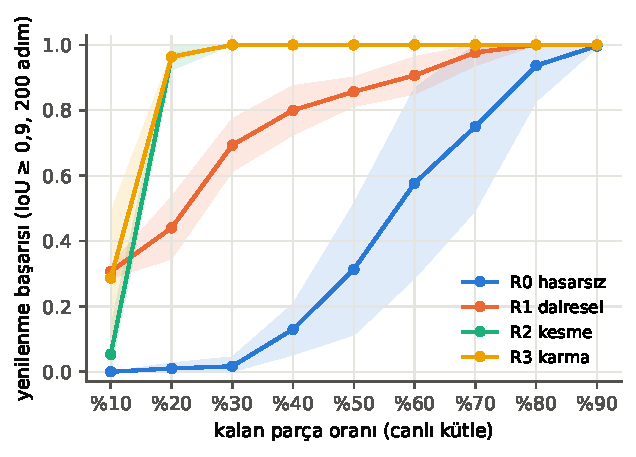
\includegraphics[width=\linewidth]{d2_fragment_curve.pdf}}{\fbox{D2 şekli: analysis/plots.py}}
\caption{Parça boyutu--yenilenme başarısı eğrisi (rejim başına, 3 tohum ortalama $\pm$ std).}
\label{fig:d2}
\end{figure}

\section{Evrimsel Katman: Ekosistem}
\subsection{Genom koşullu fizik}
% Durum [RGBA, V, gizli]; kural genomu girdi olarak okur, V'yi algılar ama değiştiremez.
% Kalıtım, yara potansiyeli V, mutasyon $g \leftarrow g + \mu V \xi$ elle yazılmış fizik (docs/evrim_tasarim.md).
\subsection{Ata eğitimi}
% Ata canlı uzayı (targets/creature_space.py): 8 genle sürekli değişen organik planaryalar; 4096 genomluk banka,
% pool + hasar, 30k iterasyon. Hedefsiz eğitim karşılaştırması: çeşitlilik renge yazıldı, şekil sabit kaldı.
\subsection{Ekoloji}
% Kaynak/enerji, gövdede hızlı enerji paylaşımı, alanla orantılı yırtıcı kesmeleri, kimlik etiketi (bireyler kaynaşmaz),
% aynı bireyle sınırlı genom homojenleşmesi, döküntü temizliği.
\subsection{Deneyler}
% E1 çeşitlilik ve canlılık; E4 parçadan yenilenme; E3 ata--torun rekabeti (gürültülü);
% E5 tek-soy uygunluk testi: kalıtsallık ve popülasyon uygunluğu eğrisi; μ taraması.
\begin{figure}[t]
\centering
\IfFileExists{../analysis/figures/e5_fitness_curve_mu.pdf}{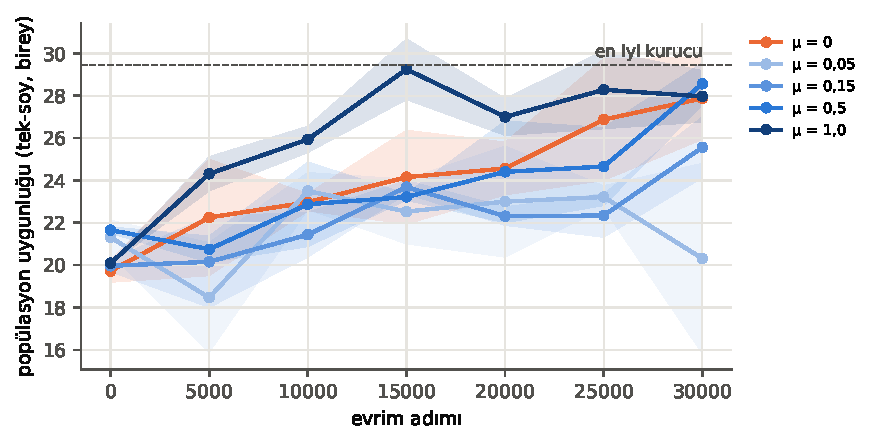
\includegraphics[width=\linewidth]{e5_fitness_curve_mu.pdf}}{\fbox{E5 şekli: analysis/plots\_evo.py}}
\caption{Popülasyon uygunluğu zaman içinde, mutasyon hızına göre (tek-soy testi, 2 tohum; gölge: standart hata). Kesikli çizgi: eğri örneklerinden en iyi kurucu (şişkin tahmin; taze tekrarlarla 25--28).}
\label{fig:e5}
\end{figure}

\section{Sonuçlar ve Tartışma}
% Seçilim işliyor (uygunluk \%30--40 artar); μ = 0,05--0,15 net yük, μ = 1 uyumu hızlandırır; doğrulama ve kesin test:
% en iyi evrimleşmiş genom 31,3 ± 2,2 vs kurucu 26,0 ± 1,9 (p = 0,08); gürültü ve kazananın laneti; ince/küçük beden seçilimi (r = −0,90).

\section{Sonuç}

\bibliographystyle{IEEEtran}
\bibliography{refs}
\end{document}
